\documentclass[a4paper, 11pt]{article}
\usepackage[utf8]{inputenc}
\usepackage[swedish]{babel}
\usepackage{hyperref}
\usepackage[margin=0.5in]{geometry}
\usepackage{graphicx}
\usepackage{amsmath}
\usepackage{textcomp} %Fuck gensymb
\usepackage{gensymb}
\usepackage[arrowdel]{physics}

\newcommand{\integ}[5][]{\int\limits_{#2}^{#3}\dd[#1]{#4}#5}
\newcommand{\del}[3][]{\partial_{#2}^{#1}#3}
\newcommand{\deval}[4][]{\dv[#1]{#2}{#3} (#4)}
\renewcommand{\var}[1]{\delta \left(#1\right)}

\title{Sammanfattning av SE1055 Hållfasthetslära}
\author{Yashar Honarmandi \\ yasharh@kth.se}
\date{\today}

\begin{document}

\maketitle

\begin{abstract}
	Denna sammanfattningen innehåller centrala definitioner och satser i SF1672 Flervariabelanalys.
\end{abstract}

\pagenumbering{roman}
\thispagestyle{empty}

\newpage

\tableofcontents

\newpage

\pagenumbering{arabic}

\section{Grundläggande definitioner för numeriska metoder}

\section{Tidsberoende problem}

\paragraph{Diskreta problem}
Betrakta ett problem där vi har $n$ punktmassor på en linje som rör sig normalt på linjens riktning, och har en förskjutning $w_{i}$ från jämviktsläget. Newtons andra lag ger
\begin{align*}
	m_{i}\ddot{w}_{i} = P_{i} - F_{i}.
\end{align*}
Här är $P_{i}$ den yttre kraften massa $i$ utsätts för och $F_{i}$ en sorts motståndsterm. Denna kan till exempel uppstå på grund av styvhet, och blir då på formen
\begin{align*}
	F_{i} = K_{ij}w_{j}.
\end{align*}
Problemet kan formuleras på matrisform som
\begin{align*}
	M\ddot{\vb{w}} + K\vb{w} = \vb{P}.
\end{align*}

Det homogena problemet kan lösas med en ansats $\vb{w} = \vb{a}\sin{\omega t}$. Detta ger upphov till ett egenvärdesproblem i egenfrekvenserna $\omega$.

Notera att 
\begin{align*}
	F_{i} = K_{ij}w_{j}.
\end{align*}
ger matrisrelationen
\begin{align*}
	\vb{F} = K\vb{w},
\end{align*}
där $K$ är styvhetsmatrisen. Vi hade alternativt kunnat ställa upp flexibilitetsmatrisen $\alpha$ för att få
\begin{align*}
	\vb{w} = \alpha\vb{F}.
\end{align*}
Det visar sig att både styvhetsmatrisen och flexibilitetsmatrisen är symmetriska.

\paragraph{Longitudinella svängningar i kontinuerliga kroppar}
Betrakta en kropp som påverkas av en normalkraft $N$ i varje ända. Snitta ut ett litet element. På ytan normal på svängningsriktningen får vi
\begin{align*}
	\rho A\dd{x}\del[2]{t}{u} = \dd{N}.
\end{align*}
Hookes lag ger
\begin{align*}
	N = EA\del{x}{u},
\end{align*}
vilket implicerar
\begin{align*}
	\rho A\del[2]{t}{u} = \del{x}{\left(EA\del{x}{u}\right)}.
\end{align*}
För en kropp med konstant styvhet $EA$ fås vågekvationen, med våghastighet
\begin{align*}
	c = \sqrt{\frac{EA}{\rho}}.
\end{align*}

\paragraph{Böjsvängningar i kontinuerliga kroppar}
Betrakta en kropp som böjs av någon utbredd last $q$. Snitta ut ett litet element. Kraftjämvikt i vertikal riktning ger
\begin{align*}
	T + \dd{T} - T + q\dd{x} = \dd{T} + q\dd{x} = \rho A\dd{x}\del[2]{t}{w} \implies \rho A\del[2]{t}{w} = q + \del{x}{T}.
\end{align*}
För låga frekvenser kan man betrakta rotationen av elementet som statisk, eventuellt inkludera en liten korrektion till egenfrekvenserna. Vi vet även från balkteori att
\begin{align*}
	\del{x}{M} = T,\ M = -EI\del[2]{x}{w}.
\end{align*}
Detta kan kombineras med resultaten ovan för att få
\begin{align*}
	\del[2]{x}{\left(EI\del[2]{x}{w}\right)} + \rho A\del[2]{t}{w} = q.
\end{align*}
Om det inte finns någon extern last och balken har konstant styvhet, reduceras detta till
\begin{align*}
	EI\del[4]{x}{w} + \rho A\del[2]{t}{w} = 0.
\end{align*}

\paragraph{Vågutbredning i kontinuerliga kroppar}
Om man gör en periodisk ansats för balkens utböjning, får man att vågtalet och frekvensen måste hänga ihop på något sätt. Detta kallas för dispersion.

\section{Balkar}

\paragraph{Elastisk vridning}
Antag att man har en stång med cirkulärt tvärsnitt fäst i ena ändan som man vrider med ett moment $M_{\text{v}}$ (i varje ända). Detta ger en vinkeldeformation $\theta$ i det yttersta tvärsnittet och $\gamma$ relativt linjen parallellt med stångens riktning. Om stången har en längd $l$ och en radius $a$, ger detta
\begin{align*}
	L\gamma = a\theta.
\end{align*}
Kombinerad med resultatet från delen om skjuvspänning ger detta
\begin{align*}
	\frac{\theta}{L} = \frac{\tau}{G}.
\end{align*}
Antag nu att $\tau = \frac{M_{\text{v}}}{K}$. Detta ger
\begin{align*}
	\frac{\theta}{L} = \frac{M_{\text{v}}}{GK}.
\end{align*}
$K$ är en konstant som beror av stångens geometri.

Hur beräknar vi $K$? Jo, man integrerar momentets differential över tvärsnittet. Vi vet att detta differentialet ges av kraft gånger arm, och det är så skjuvspänningen kommer in.

\paragraph{Balkböjning - fundamentala koncept}
För att beskriva balkar behöver vi införa fler olika sorters inre krafter och moment. Dessa illustreras i figur \ref{fig:beam_forces}.
\begin{figure}[!ht]
	\centering
	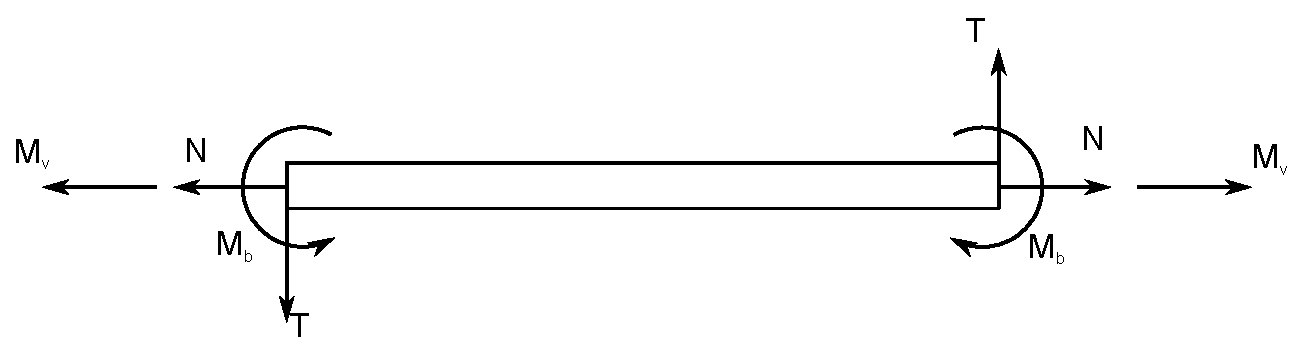
\includegraphics[width = 0.5\textwidth]{./Images/beam_forces.eps}
	\caption{Illustration av inre krafter och moment i en balk.}
	\label{fig:beam_forces}
\end{figure}
Vi har infört normalkraften $N$, tvärkraften $T$, det böjande momentet $M_{\text{b}}$ och det vridande momentet $M_{\text{v}}$.

Låt $u$ vara balkens deformation normalt på dens utsträkning. Vi har från enaxliga tillståndet att
\begin{align*}
	\frac{\Delta u}{L} = \frac{N}{EA}.
\end{align*}
Låt $\theta$ och $\phi$ vara vinklarna för böjning och vridning. Vi har från innan att
\begin{align*}
	\frac{\Delta\theta}{L} = \frac{M_{\text{v}}}{GK},
	\frac{\Delta\phi}{L} = \frac{M_{\text{b}}}{EI}.
\end{align*}

\paragraph{Allmänt tillstånd för en balk}
Snitta nu ut ett element med längd $\dd{x}$ från en balk. Om balken påverkas av en last $q$ per längdenhet, ger kraftjämvikten
\begin{align*}
	T(x + \dd{x}) - T(x) + q(x)\dd{x} = 0,
\end{align*}
vilket ger
\begin{align*}
	\dv{T}{x} = -q.
\end{align*}
Momentjämvikt kring centrum ger
\begin{align*}
	M(x + \dd{x}) - M(x) - (T(x) + T(x + \dd{x}))\dd{x} = 0.
\end{align*}
Bidraget från tvärkraften ges av
\begin{align*}
	T(x) + T(x + \dd{x}) &= 2T(x) + \dv{T}{x}\dd{x} \\
	                     &= 2T(x) - q(x)\dd{x}.
\end{align*}
Insatt i momentjämvikten fås
\begin{align*}
	M(x + \dd{x}) - M(x) - \frac{1}{2}\dd{x}(T(x) + T(x + \dd{x})) = M(x + \dd{x}) - M(x) - T(x)\dd{x} + \frac{1}{2}\dd{x}q(x)\dd{x}.
\end{align*}
Vi försummar nu alla andra ordningens termer, vilket ger
\begin{align*}
	\dv{M}{x} = T.
\end{align*}
Kombinerat med det förra resultatet fås
\begin{align*}
	\dv[2]{M}{x} = -q.
\end{align*}

\paragraph{Randvillkor för balkar}
En balk kan i en given ända vara
\begin{itemize}
	\item fri, vilket ger $T = 0$ och $M = 0$.
	\item fritt upplagd, vilket ger $M = 0$.
	\item glidinspänd, vilket ger $T = 0$.
	\item fast inspänd, vilket ej ger villkor för de inre krafterna och momenterna.
\end{itemize}

\paragraph{Balkböjning vid normalspänning}
Vid böjning inför vi en $z$-koordinat normal på medellinjen genom balken, och centrerar våra koordinater i tvärsnittets tyngdpunkt. Vi antar till att börja med att tvärsnittet är symmetrisk med avseende på $z$-axeln, samt att
\begin{itemize}
	\item plana tvärsnitt förblir plana.
	\item tvärsnitt förblir vinkelräta mot medellinjen.
	\item det för varje $z$ är ett enaxligt samband mellan $\sigma$ och $\varepsilon$.
	\item alla deformationer är små och för balkar vars längd är mycket större än deras tjocklek.
\end{itemize}
De två första uppfylls om skjuvspänningen är försumbar jämförd med normalspänningen.

Betrakta nu ett litet element med ursprunglig längd $L_{0}$ vars medellinje har böjts så den har krökningsradie $R$. Geometri ger oss
\begin{align*}
	(R + z)\phi = L_{0}(1 + \varepsilon(z)).
\end{align*}
I $z = 0$ har vi
\begin{align*}
	R\phi = L_{0}(1 + \varepsilon_{0}),
\end{align*}
vilket ger
\begin{align*}
	L_{0}(1 + \varepsilon_{0}) + z\phi &= L_{0}(1 + \varepsilon(z)), \\
	\varepsilon(z)                     &= \varepsilon_{0} + \frac{\phi}{L_{0}}z.
\end{align*}
Vi kan även substituera för $\phi$ för att få
\begin{align*}
	\varepsilon(z) = \varepsilon_{0} + \frac{1 + \varepsilon_{0}}{R}z.
\end{align*}

Om vi snittar och får någon given normalkraft $N$ på ytan, gäller det att
\begin{align*}
	N &= \integ{A}{}{F}{} \\
	  &= \integ{A}{}{A}{\sigma}.
\end{align*}
Hookes lag ger
\begin{align*}
	N &= \integ{A}{}{A}{E\left(\varepsilon_{0} + \frac{z}{R}\right)} \\
	  &= \integ{A}{}{A}{E\varepsilon_{0} + E\frac{z}{R}}.
\end{align*}
Om vi antar att elasticitetsmodulen är konstant över ytan, kan vi dra ut konstanter. Den andra integralen är då tyngdpunktens $z$-koordinat (om vi antar homogen massfördelning), som per definition var $0$. Detta ger
\begin{align*}
	N = E\varepsilon_{0}A.
\end{align*}

Vi beräknar vidare det böjande momentet $M_{y}$, som är normalt på både längdriktningen och $z$-koordinaten. Detta ges av
\begin{align*}
	M_{y} &= \integ{A}{}{A}{\sigma z} \\
	      &= \integ{A}{}{A}{Ez\left(\varepsilon_{0} + \frac{z}{R}\right)} \\
	      &= \integ{A}{}{A}{Ez\varepsilon_{0} + \frac{E}{R}z^{2}}.
\end{align*}
Första integralen är igen lika med $0$. Andra är relaterad till yttröghetsmomentet
\begin{align*}
	I_{y} = \integ{A}{}{A}{z^{2}}.
\end{align*}
Vi får alltså
\begin{align*}
	M_{y} = \frac{EI_{y}}{R}.
\end{align*}
Vi kan nu sätta ihop dessa resultat och få
\begin{align*}
	\sigma = \frac{N}{A} + \frac{M_{y}}{I_{y}}z.
\end{align*}

Vid ren böjning, dvs. ingen normalkraft, kan vi skriva
\begin{align*}
	\abs{\sigma}_{\text{max}} = \frac{\abs{M_{y}}\abs{z}_{\text{max}}}{I_{y}}.
\end{align*}
Vi kan införa böjmotståndet
\begin{align*}
	W_{\text{b}} = \frac{I_{y}}{\abs{z}_{\text{max}}},
\end{align*}
och får då
\begin{align*}
	\abs{\sigma}_{\text{max}} = \frac{\abs{M_{y}}}{W_{\text{b}}}.
\end{align*}

\paragraph{Allmänt tillstånd för en balk}
Vi försöker nu sammanställa dessa resultat till ett allmänt tillstånd för balken.

Geometri ger oss att
\begin{align*}
	\frac{1}{\abs{R}} = \frac{\dv[2]{u}{x}}{\left(1 + \left(\dv{u}{x}\right)^{2}\right)^{\frac{3}{2}}}.
\end{align*}
För små deformationen är derivatan mycket liten. Om vi definierar positiv krökning som att balken kröks nedåt, fås
\begin{align*}
	\frac{1}{R} = -\dv[2]{u}{x}.
\end{align*}
Materialsamband ger
\begin{align*}
	M_{\text{b}} = -EI_{y}\dv[2]{u}{x}.
\end{align*}
Vi har även
\begin{align*}
	\dv[2]{M_{\text{b}}}{x} = -q,
\end{align*}
vilket slutligen ger
\begin{align*}
	\dv[2]{x}\left(EI_{y}\dv[2]{u}{x}\right) = q.
\end{align*}

Till detta tillståndet hör olika sorters randvillkor. Några enkla varianter av randvillkor är
\begin{itemize}
	\item $u$ eller $T$ givna i ändpunkterna.
	\item $\dv{u}{x}$ eller $M$ givna i ändpunkterna.
\end{itemize}
Vi kan även karakterisera ändpunkter som
\begin{itemize}
	\item fria, dvs. $T = 0$ och $M = 0$.
	\item fritt upplaggda, dvs. $u = 0$ och $M = 0$.
	\item fast inspända, dvs. $u = 0$ och $\dv{u}{x} = 0$.
	\item glidande inspända, dvs. $\dv{u}{x} = 0$ och $T = 0$.
\end{itemize}

\paragraph{Superposition}
Balkens allmänna tillstånd är linjärt, så om man har någon komplicerad sammansättning av yttre laster och krafter, kan man separera problemet i olika delproblem, lösa de separat och superponera lösningen.

\paragraph{Plasticering av balk}
Betrakta en balk som endast utsätts för ett böjmoment $M$. Vid inledande plasticering är
\begin{align*}
	\sigma_{\text{max}} = \sigma_{\text{s}}.
\end{align*}
Vi vet i detta fallet att
\begin{align*}
	\sigma_{\text{max}} = \frac{\abs{M}}{W_{\text{b}}},
\end{align*}
vilket ger
\begin{align*}
	M_{\text{s}} = W_{\text{b}}\sigma_{\text{s}}.
\end{align*}

Vid full plasticering är spänningen lika med $\sigma_{\text{s}}$ i hela balken. Från detta kan man beräkna böjmomentet. Som ett exempel fås för ett rektangulärt tvärsnitt som böjs i höjdriktning:
\begin{align*}
	M_{\text{f}} = 2\cdot\sigma_{\text{s}}b\frac{h}{2}\cdot\frac{h}{4}.
\end{align*}
Man kan även visa att detta är lika med $\frac{3}{2}M_{\text{s}}$.

Vid avlastning kan man använda superposition för att få spänningstillståndet. Det kommer visa sig att restspänningen är diskontinuerlig i mitten.

\paragraph{Tillstånd för axialbelastad balk}
Betrakta en balk som utsätts för en axial belastning, och snitta ut ett element i den enligt figur \ref{fig:skew_beam_forces}.
\begin{figure}
	\centering
	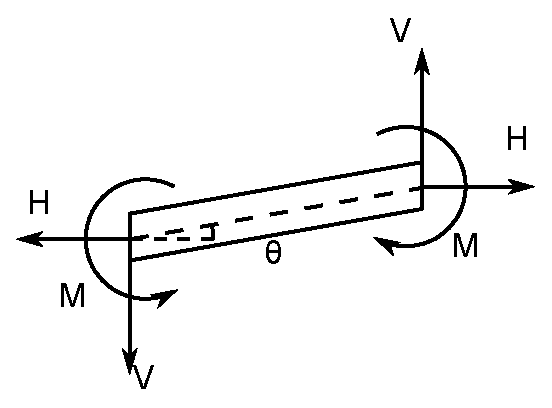
\includegraphics[width = 0.5\textwidth]{./Images/skew_beam_forces.eps}
	\caption{Snitt i en axialbelastad balk, där snittet görs vertikalt relativt det odeformerade läget.}
	\label{fig:skew_beam_forces}
\end{figure}
Kraft- och momentjämvikter ger
\begin{align*}
	V(x + \dd{x}) - V(x) + q\dd{x} = 0, \\
	H(x + \dd{x}) - H(x) = 0, \\
	M(x + \dd{x}) - M(x) - V(x)\dd{x} + H\dv{w}{x}\dd{x} = 0,
\end{align*}
där vi har utnyttjat att vinkeln $\theta$ ges av derivatan av utböjningen och försummat det andra ordningens bidraget till momentet från den utbrädda lasten. Detta ger
\begin{align*}
	\dv{V}{x} = -q,\ \dv{H}{x} = 0,\ \dv{M}{x} = V - H\dv{w}{x}.
\end{align*}
Man kan visa att till första ordningen är $H = N$, och $N$ ges av den yttre axiala lasten (och eventuella volymkrafter). Kombinationen av dessa ekvationer ger då
\begin{align*}
	\dv[2]{x}\left(EI\dv[2]{w}{x}\right) - N\dv[2]{w}{x} = 0.
\end{align*}

\input{./Parts/energy_methods.tex}

\section{Finita elementmetoden}

Finita elementmetoden (FEM) är en metod för att numeriskt lösa partiella differentialekvationer. Den kan tillämpas på problem inom allt från strömningmekanik och hållfasthetslära till kvantmekanik.

Grunden för FEM är att lösa problem med hjälp av potentiella energins minimum. Vi kunde formulera en potential $U = W_{\text{e}} - A$, där
\begin{align*}
	W_{\text{e}} = \integ{0}{l}{x}{\frac{1}{2}EA\left(\dv{u}{x}\right)^{2}}
\end{align*}
för en balk och
\begin{align*}
	A = \integ[3]{0}{l}{x}{K} + \sum F_{i}u(x_{i}
\end{align*}
är bidraget från yttre krafter. För att hitta en approximativ lösning, gör man ansatsen
\begin{align*}
	u = \sum a_{i}f_{i},
\end{align*}
där alla $f_{i}$ är kända. Nu kommer potentialen bero av de olika koefficienterna, och att minimera potentiella energin innebär nu att hitta koefficienter i summan så att potentiella energin minimeras. I FEM använder man speciella val av såna ansatsfunktioner.

Mer specifikt diskretiserar man först problemet, och skriver
\begin{align*}
	u(x) = \sum d_{i}N_{i}(x)
\end{align*}
där $d_{i}$ är förskjutningen i den $i$:te punkten och $N_{i}$ är formfunktioner. Ett enkelt val av formfunktioner är $N_{i}(x_{j}) = \delta_{ij}$. Denna summan kan man alternativt skriva som en skalärprodukt $u = Nd = d^{T}N^{T}$, där $N$ är en radvektor med alla $N_{i}$ och $d$ en kolumnvektor med alla $d_{i}$. Vi måste även införa $B = \dv{N}{x}$ Nu kan vi skriva potentiella energin som
\begin{align*}
	U &= \integ{0}{l}{x}{\frac{1}{2}d^{T}B^{T}EABd - K_{x}d^{T}N^{T}} - \sum F_{i}d^{T}N^{T} \\
	  &= \frac{1}{2}d^{T}Kd - d^{T}F
\end{align*}
där vi har infört styvhetsmatrisen
\begin{align*}
	K = \integ{0}{l}{x}{\frac{1}{2}B^{T}EAB}
\end{align*}
och matrisen
\begin{align*}
	F = \integ{0}{l}{x}{K_{x}N^{T}} - \sum F_{i}N^{T}.
\end{align*}
Potentiella energins minimum ges då av
\begin{align*}
	Kd - F = 0.
\end{align*}

\section{Materialers beteende}

\paragraph{Idealplastisk deformation}
De flesta material beter sig så att när de deformeras förbi en viss punkt, deformeras de plastiskt i stället för elastiskt. En approximation för att beskriva detta beteendet är att låta deformationen vara elastisk upp till en töjningsgräns $\varepsilon_{\text{s}}$, och låta $\sigma$ vara konstant lika med en sträckgräns $\sigma_{\text{s}}$ för större töjningar.

När lasten sedan tas bort, kommer stången förkortas igen tills lasten blir lika med noll. Denna kontraktionen är parallell med det elastiska regimet, och konsekvensen är att man får en permanent deformation.

\paragraph{Enkelriktad fiberkomposit}
En enkelriktad fiberkomposit är ett material som består av fibrar som alla är parallella och ett omkransande material som kallas en matris. Matrisen och fibern finns i volymfraktioner $v_{\text{m}}$ respektiva $v_{\text{f}}$, och de har elasticitetsmoduler $E_{\text{m}}$ respektiva $E_{\text{f}}$.

Som en modell för belastning längsmed fibrernas riktning betraktar vi uppställningen som ges i figur \ref{fig:fiber_composite_parallel}.
\begin{figure}[!ht]
	\centering
	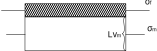
\includegraphics[width = 0.5\textwidth]{./Images/fiber_composite_parallel.eps}
	\caption{Illustration av en del av en enkelriktad fiberkomposit som belastas längsmed fiberns riktning.}
	\label{fig:fiber_composite_parallel}
\end{figure}

Kraftjämvikten ger $F = \sigma A$. Vi antar att den utskurna biten är ett rätblock, så de två delarna har tvärsnittsareor som ges av totala tvärsnittsarean och volymfraktionerna. Detta ger
\begin{align*}
	F = \sigma A = (\sigma_{\text{f}}v_{\text{f}} + \sigma_{\text{m}}v_{\text{m}})A.
\end{align*}
Därmed ges spänningen av
\begin{align*}
	\sigma = \sigma_{\text{f}}v_{\text{f}} + \sigma_{\text{m}}v_{\text{m}}.
\end{align*}
Vi antar att fibern och matrisen inte glider relativt varandra, och därmed har de samma deformation och töjning. Hookes lag ger
\begin{align*}
	\sigma_{\text{f}} = E_{\text{f}}\varepsilon, \sigma_{\text{m}} = E_{\text{m}}\varepsilon,
\end{align*}
vilket insatt i uttrycket ovan ger
\begin{align*}
	\sigma &= v_{\text{f}}E_{\text{f}}\varepsilon + v_{\text{m}}E_{\text{m}}\varepsilon \\
	       &= (v_{\text{f}}E_{\text{f}} + v_{\text{m}}E_{\text{m}})\varepsilon.
\end{align*}
För hela biten med fiberkomposit ger Hookes lag då
\begin{align*}
	E_{\text{L}} = v_{\text{f}}E_{\text{f}} + v_{\text{m}}E_{\text{m}}
\end{align*}
som elasticitetsmodulen vid längsgående spänning. Vi får även
\begin{align*}
	\sigma_{\text{f}} &= E_{\text{f}}\varepsilon \\
	                  &= \frac{E_{\text{f}}}{E_{\text{L}}}\sigma
\end{align*}
som spänning i fibrerna, och motsvarande för matrisen.

På samma sättet beskriver vi även fallet när spänningen går på tvärs av fibrernas riktning, som illustrerad i figur \ref{fig:fiber_composite_normal}.
\begin{figure}[!ht]
	\centering
	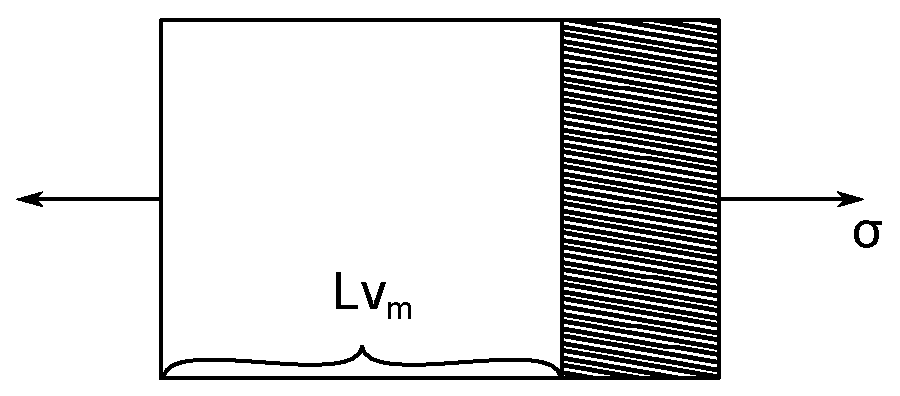
\includegraphics[width = 0.5\textwidth]{./Images/fiber_composite_normal.eps}
	\caption{Illustration av en del av en enkelriktad fiberkomposit som belastas normalt på fiberns riktning.}
	\label{fig:fiber_composite_normal}
\end{figure}

Här kan vi snitta och se att $\sigma_{\text{f}} = \sigma_{\text{m}}$. Den totala förlängningen i denna biten ges av
\begin{align*}
	\delta = \delta_{\text{f}} + \delta_{\text{m}} = L_{\text{f}}\varepsilon_{\text{f}} + L_{\text{m}}\varepsilon_{\text{m}}.
\end{align*}
Töjningen ges då av
\begin{align*}
	\varepsilon &= \frac{\delta}{L_{\text{f}} + L_{\text{m}}} \\
	            &= \varepsilon_{\text{f}}\frac{L_{\text{f}}}{L_{\text{f}} + L_{\text{m}}} + \varepsilon_{\text{m}}\frac{L_{\text{m}}}{L_{\text{f}} + L_{\text{m}}} \\
	            &= v_{\text{f}}\varepsilon_{\text{f}} + v_{\text{m}}\varepsilon_{\text{m}}.
\end{align*}
Hookes lag ger
\begin{align*}
	\varepsilon &= v_{\text{f}}\frac{\sigma}{E_{\text{f}}} + v_{\text{m}}\frac{\sigma}{E_{\text{m}}},
\end{align*}
och vi ser att
\begin{align*}
	\frac{1}{E_{T}} = \frac{v_{\text{f}}}{E_{\text{f}}} + \frac{v_{\text{m}}}{E_{\text{m}}}.
\end{align*}

\paragraph{Ideallastisk vridning}
Vi inför idealplastiska material även i vridningssammanhang. Dessa beter sig analogt till idealplastiska material under dragning, där vi ersätter töjningen med skjuvvinkeln $\gamma$, spänningen med skjuvspänningen $\tau$, töjningsgränsen med en vinkelgräns $\gamma_{\text{s}}$ och sträckgränsen med en skjuvgräns $\tau_{\text{s}}$.

\paragraph{Knäckning}
Om man t.ex. belastar en balk i dens längdriktning med en last som är större än en viss kritisk last, kommer balken snabbt böjas och nå ett nytt jämviktsläge. Detta kommer av att ursprungsläget är en instabil jämviktspunkt, så den minsta störning kommer att få den att anta ett stabilt jämviktstillstånd. Detta är ett exempel på ett instabilitetsfenomen.

\paragraph{Plasiticitetsteori i tre dimensioner}
I tre dimensioner inför vi effektivspänningen $\sigma_{\text{e}}$, som beror av spänningsmatrisen, och kräver $\sigma_{\text{e}}(S) = \sigma_{\text{s}}$ för att plasticitet skall inträda. Vi kommer undersöka detta för isotropa material.

Vi kan välja huvudspänningsriktningarna som koordinatsystem. Då kan effektivspänningen reduceras till $\sigma_{\text{e}}(S) = \sigma_{\text{e}}(\sigma_{1}, \sigma_{2}, \sigma_{3})$. Plasticitetskriteriet definierar då en yta i tre dimensioner. Av rimlighetsskäl kan ytan inte skära origo.

Vi kan kräva vissa saker av flytvillkoret, till exempel
\begin{itemize}
	\item det skall vara oberoende av eventuellt hydrostatiskt tryck, dvs. $\sigma_{\text{e}}(\sigma_{1}, \sigma_{2}, \sigma_{3}) = \sigma_{\text{e}}(\sigma_{1} - p, \sigma_{2}- p, \sigma_{3}- p) = \sigma_{\text{s}}$. Detta implicerar att ytan som definieras av flytvillkoret är en cylinderyta med riktning $(1, 1, 1)$.
	\item det uppfyller ett enaxligt flytvillkor, dvs. att om någon huvudspänning är $\sigma_{\text{s}}$ och de andra är $0$, uppfylls flytvillkoret.
	\item det är oberoende av reversering av spänningstillståndet, dvs. om alla huvudspänningar byter tecken är flytvillkoret uppfyld.
	\item det är isotropiskt, dvs. permutation av huvudspänningarna ger fortfarande att flytvillkoret är uppfyld.
\end{itemize}
Från detta kan vi dra slutsatsen att vi endast behöver titta på en $30\degree$ sektor av ytan, då symmetrier ger resten av ytan.

\paragraph{von Mises}
von Mises lösning är att säja att denna sektorn är en cirkelbåge. Det finns en formel för denna.

\paragraph{Tresca}
Trescas lösning är att säja att denna sektorn är en rät linje. Det finns en formel för denna.

\paragraph{Jämförelse}
Om man jämför Trescas och von Mises teorir, blir det störst skillnad vid ren vridning. Trescas villkor är en mer konservativ gräns än von Mises, då den allmänt ligger närmare origo. Trescas villkor har hörn, och är därför svår numeriskt. Båda funkar ändå rätt bra när man jämför med experiment.

\paragraph{Utmattning}
Utmattning är fenomenet som uppstår när brott uppstår under spänningsgränser. Det som händer är att spänningsgränsen blir lägre i materialet av cyklisk deformation, och att den tenderer mot en utmattningsgräns.

För att beskriva cykliska belastningar, inför vi begreppen minimumspänning, maximumspänning, amplitudspänning, mittspänning och spänningsförhållande. Vi har
\begin{align*}
	\sigma_{\text{a}} &= \frac{\sigma_{\text{max}} - \sigma_{\text{min}}}{2}, \\
	\sigma_{\text{m}} &= \frac{\sigma_{\text{max}} + \sigma_{\text{min}}}{2}, \\
	R                 &= \frac{\sigma_{\text{min}}}{\sigma_{\text{max}}}.
\end{align*}

\paragraph{Dragprovning och S-N-diagram}
För att testa materialers utmattningsegenskaper, kan man utsätta ett prov för varierande spänningar. Det vanlige är rent varierande eller pulserande spänningar. För en given spänningsamplitud kan man mäta hur många cykler provet kan gå igenom innan brott, och detta kan plottas i ett S-N-diagram. I ett sånt diagram kan man också rita olika kurvor för olika brottsannolikheter.

Av detta kan man läsa av brottgränsen $\sigma_{\text{B}}$ vid låga $N$ och utmattningsgränsen $\sigma_{\text{u}}$ vig höga $N$. Om man belastar provet med en spänning som är lägre än detta, har provet oändlig livslängd. Kurvan har typiskt en omvänd sigmoid form, och gränslivslängden $N{\text{g}}$ definieras som det $N$ där kurvan igen blir platt. Om spänningen är pulserande, betacknas utmattningsgränsen som $\sigma_{\text{up}}$. Motsvarande gränser kan även införas vid böjning eller böjning med rotation.

\paragraph{Haigh-diagram}
Ett Haigh-diagram är en representation av alla kombinationer av mittspänning och amplitudspänning som ger brott. Vi kommer dock förhålla oss till förenklade Haigh-diagram. Dessa konstrueras vid att dra räta linjer mellan olika punkter.

Den första punkten är $\sigma_{\text{m}} = 0, \sigma_{\text{a}} = \sigma_{\text{u}}$, som motsvarar rent växlande belastning. Den andra punkten är en rent växlande spänning $\sigma_{\text{a}} = \sigma_{\text{m}} = \sigma_{\text{up}}$. Den tredje punkten fås från ett rent statiskt dragprov $\sigma_{\text{a}} = 0, \sigma_{\text{m}} = \sigma_{\text{B}}$. Linjerna mellan dessa är ett Haigh-diagram. Man kan även förfina vid att lägga till en linje mellan $\sigma_{\text{s}}$ på båda axlarna för att ta höjd för plasticering. Då blir Haigh-diagrammet den kurvan som ligger lägst i diagrammet.

För att undersöka om den givna lasten ger brott, ritar man punkten in i Haigh-diagrammet. Om punkten är under kurvan, sker inte brott.

\paragraph{Dimensionering}
I vanliga fall vill man inte göra val baserad på gränserna utan med lite marginaler. Då kan man välja efter gränserna, fast multiplicerad med en faktor
\begin{align*}
	1 - \frac{\lambda}{K_{\text{f}}K_{\text{r}}K_{\text{d}}}.
\end{align*}
De olika faktorerna här förtjäner lite förklaring.

$\lambda$ är en faktor som tillkommer på grund av materialkvalitet. I moderna material är denna endast viktig för gjutna komponenter.

$K_{\text{f}}$ beror igen av en geometrisk faktor $K_{\text{t}}$. Tack, hållf. Om det finns variationer i komponentens tvärsnitt längsmed dens längd, beräknar man nominell spänning med hjälp av den minsta tvärsnittsdatan för att uppskatta den största spänningen som förekommer. Den maximala spänningen i komponenten är dock större än detta, tydligen, och kvoten mellan den maximala och nominella spänningen är $K_{\text{t}}$. $K_{\text{f}}$ fås med hjälp av sambandet $K_{\text{f}} = 1 + q(K_{\text{t}} - 1)$, där $q$ är en materialberoende storhet.

$K_{\text{r}}$ beskriver ytfinheten, som visar sig påverka hållfastheten. Denna beror igen av medelytavvikelsen $R_{\text{a}}$.

$K_{\text{d}}$ beror av provets storlek. Storleken spelar in på ett sätt som inte är helt klart.

När man nu har konstruerat sitt förbättrade Haigh-diagram, kan man bestämma säkerhetsfaktorer med hjälp av avstånd i Haigh-diagrammet. Hur detta görs beror på vilken sorts last man har, och beskrivs (förhoppningsvis) i formelbladet.

\end{document}
